\documentclass[twoside,10pt]{article}
\usepackage{shlists}
\usepackage[applemac]{inputenc}
\usepackage[spanish]{babel}
\usepackage[T1]{fontenc}


\usepackage{multicol}
\usepackage{picinpar}

\usepackage{url}
\newcommand{\surl}[1]{{\small\url{#1}}}

\newcounter{vol}
\newcounter{num}
\newcounter{anyo}
\setcounter{vol}{9}
\setcounter{num}{2}
\setcounter{anyo}{2016}
\newcommand{\mes}{Mayo}
\usepackage{revisionNLcol}


\title{\ \\ Docencia 2.0\\ \large Juan Juli\'{a}n Merelo, Fernando Tricas}
\author{\LARGE En defensa de los trabajos de fin de grado}

\date{}

\AutTit{Docencia 2.0}

\begin{document}
\addtocounter{page}{2}

\maketitle
\vspace*{-5ex}

\begin{multicols}{2}
 
Recientemente, con la transformaci\'{o}n de los t\'{\i}tulos universitarios con
la convergencia al espacio europeo de educaci\'{o}n superior se est\'{a}n
escuchando cr\'{\i}ticas a la necesidad de realizar trabajos de fin de
Grado y M\'{a}ster (TFG/TFM). Sobre todo en titulaciones donde no exist\'{\i}a la
costumbre y se est\'{a}n enfrentando a las complejidades del dise\~{n}o de este
tipo de asignaturas. Simult\'{a}neamente, en las comisiones de acreditaci\'{o}n se
pide que se incluya la nota obtenida por los alumnos a los que se les ha
dirigido tal trabajo, convirti\'{e}ndolos de esa forma, en
una manera m\'{a}s de evaluar al docente en ciertas instancias. 

Queremos dedicar estas l\'{\i}neas a las ventajas que vemos a este tipo de
trabajo que culminan unos estudios y que deber\'{\i}an verse, por muchos
motivos, como un paso importante en vez de una molestia innecesaria
e inevitable, todo ello desde la experiencia de llevar unos cuantos
a\~{n}os impartiendo docencia en titulaciones de ingenier\'{\i}a, donde el
proyecto de fin de carrera y luego los TFG/TFM son una
costumbre establecida. Aportamos la experiencia de haber dirigido unos cuantos
de estos trabajos y formado parte de otro buen n\'{u}mero de tribunales
evaluadores. Del viejo, el consejo. Y de unas personas que han estado en m\'{a}s
tribunales de trabajos que Eva Hache en los de Got Talent, una serie de
valoraciones sobre los mismos. 

En el principio, eran las {\em tesinas}. Un trabajo, extenso,
posiblemente m\'{a}s acad\'{e}mico que otra cosa, que se presentaba con
chaqueta y corbata ante un serio tribunal de la c\'{a}tedra m\'{a}s pr\'{o}xima a
la carrera. En las ingenier\'{\i}as, las tesinas devinieron
proyectos.
 Y los proyectos, eventualmente, se convirtieron en trabajos,
 perdiendo ese aura vital de algo que se emprende, que avanza. Un
 trabajo es algo que hay que entregar, pero que puede tener o no que
 ver con tu vida, o tu trabajo, {\em real}. 

A\'{u}n as\'{\i}, con su extensi\'{o}n a muchos grados, un trabajo fin de grado o
TFG es algo que est\'{a} m\'{a}s relacionado con la madurez del alumno que con
sus conocimientos t\'{e}cnicos; es transversal en el sentido que tiene que
servir no tanto para adquirir conocimientos t\'{e}cnicos, sino para ponerlos
en pr\'{a}ctica en una situaci\'{o}n tan del mundo real como el tutor y el
alumno puedan permitirse.  Por eso, desde el punto de vista del
alumno y siguiendo el adagio �Del viejo, el consejo�, convendr\'{\i}a
tener en cuenta las siguientes ideas

Todos tenemos m\'{u}ltiples facetas en la vida y frases de \'{a}nimo que nos
pueden ayudar en este duro trance. Empezando por {\sl Party hard, work
  hard}. Seguro que nuestros allegados ya tienen claro que nos 
defendemos con mayor o menor acierto cuando toca divertirse. El trabajo de fin
de (estos) estudios debe (o al menos puede) ser un trabajo que re\'{u}na una parte
considerable de los conocimientos alcanzados en los mismos. Tambi\'{e}n debe (o
puede) permitirnos explorar algunos temas laterales que no se hayan tratado de
manera completa en lo estudios regulares, o temas novedosos con 
cierto ``riesgo''
que no sabemos si llegar\'{a}n a alcanzar la consolidaci\'{o}n dentro de la
disciplina. Las ense\~{n}anzas regladas son eso, regladas. En estos trabajos  se
  invita al alumno que se salte un poco las reglas. As\'{\i} que {\sl Party
    on!}
	
%--------------------------
\noindent\rule{86mm}{1pt}
\vspace{1ex} {\small{\begin{window}[0,r,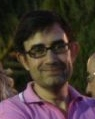
\includegraphics[width = 27mm]{JJM.jpg},] 
\noindent\emph{JJ Merelo} es catedr\'{a}tico de Universidad
en el \'area de Arquitectura y Tecnolog\'{\i}a de Computadores, y
actualmente director de la Oficina de Software Libre de la UGR.
Mantiene un blog desde el a\~no 2002, y lo ha utilizado en clase desde
el a\~no 2004; tambi\'en wikis, agregadores y repositorios de c\'odigo
como herramientas docente. \'{U}ltimamente le ha dado por el \textsl{flipped
learning}, de lo que se informar\'{a} debidamente en esta columna.
\end{window}}}

\medskip

{\small{\begin{window}[0,r,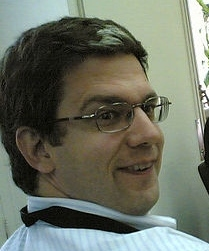
\includegraphics[width = 27 mm]{FTricas1.jpg},]
		\noindent \emph{Fernando Tricas Garc\'{\i}a} es profesor
		titular de Lenguajes y Sistemas Inform\'{a}ticos del Departamento
		de Inform\'{a}tica e Ingenier\'{\i}a de Sistemas de la Universidad de
		Zaragoza.  Empez\'{o} a estudiar la blogosfera casi cuando a\'{u}n no
		exist\'{\i}a (all\'{a} por el a\~{n}o 2002) y a tratar de integrarla en los
		cursos y tareas docentes un poco despu\'{e}s.  Ha impartido
		numerosas charlas relacionadas con el tema de la Web 2.0, 
		internet y universidad,\ldots\ 
		Es actualmente Vicerrector de Tecnolog\'{\i}as de la Informaci\'{o}n y
de la Comunicaci\'{o}n.   
		\end{window}}}
%-------------------------------------------------

		

% %--------------------------
% \begin{figure}[b]
% \rule{86mm}{1pt}
% \begin{minipage}[c]{\textwidth}
% {\small{\begin{window}[0,r,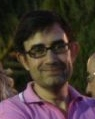
\includegraphics[width=27mm]{JJM.jpg},] 
%       \noindent\emph{JJ Merelo} es catedr\'{a}tico de Universidad
%       en el \'{a}rea de Arquitectura y Tecnolog\'{\i}a de Computadores, y
%       actualmente director de la Oficina de Software Libre de la UGR.
%       Mantiene un blog desde el a\~{n}o 2002, y lo ha utilizado en clase desde
%       el a\~{n}o 2004; tambi\'{e}n wikis, agregadores y repositorios de c\'{o}digo
%       como herramienta docente. \'{U}ltimamente le ha dado por el \textsl{flipped
%         learning}, de lo que se informar\'{a} debidamente en esta columna.
%     \end{window}}}
% \end{minipage}
% 
% \begin{minipage}[c]{\textwidth}
% {\small{\begin{window}[0,r,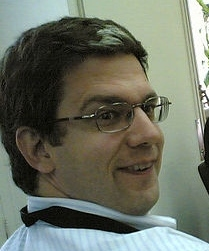
\includegraphics[width = 27 mm]{FTricas1.jpg},]
% 		\noindent  \emph{Fernando Tricas Garc\'{\i}a} es profesor
% 		titular de Lenguajes y Sistemas Inform\'{a}ticos del Departamento
% 		de Inform\'{a}tica e Ingenier\'{\i}a de Sistemas de la Universidad de
% 		Zaragoza.  Empez\'{o} a estudiar la blogosfera casi cuando a\'{u}n no
% 		exist\'{\i}a (all\'{a} por el a\~{n}o 2002) y a tratar de integrarla en los
% 		cursos y tareas docentes un poco despu\'{e}s.  Ha impartido
% 		numerosas charlas relacionadas con el tema de la Web 2.0, internet y universidad, ...
% 		Es actualmente Vicerrector de Tecnolog\'{\i}as de la Informaci\'{o}n y
% de la Comunicaci\'{o}n.  
% 		\end{window}}}
% \end{minipage}
% \end{figure}
% %-------------------------------------------------

\noindent Salt\'{a}ndonos las reglas, podemos llevar a cabo uno de
nuestros sue\~{n}os. Porque {\sl If you can dream it, you can do it}. Salvo que tengamos un
  marcado esp\'{\i}ritu emprendedor el trabajo de fin de estudios puede ser
  una de las \'{u}ltimas veces en las que podamos tomar nuestras propias
  decisiones sobre lo que queremos trabajar. Luego iremos a trabajar
  en el ``mundo real''\textregistered\  y all\'{\i} pasaremos una temporada
  haciendo lo que seguramente decidir\'{a}n otros. En un proyecto, t\'{u} eres
  literalmente el jefe de proyecto, el responsable del mismo. La
  experiencia que tengas dirigi\'{e}ndote a ti mismo te puede ser \'{u}til si,
  m\'{a}s adelante, tienes que dirigir a alguien. 

Pero lo esencial es demostrarte que realmente puedes llevar a cabo un
proyecto completo, como un ingeniero: {\sl Yes we can}. Despu\'{e}s de unos cuantos a\~{n}os estudiando podremos
  demostrar (y demostrarnos) que somos capaces de abordar un proyecto
  m\'{a}s o menos grande (no tan grande, en realidad) pasando por diversos
  procesos que hemos aprendido en nuestros estudios: investigar,
  analizar, examinar alternativas, tomar decisiones y asumir sus
  consecuencias. S\'{\i}, podemos, pero tambi\'{e}n podemos equivocarnos y una
  refactorizaci\'{o}n a un mes de la entrega te puede ense\~{n}ar tanto como
  varias asignaturas de ingenier\'{\i}a del \textsl{software} juntas. 

Como puede hacerlo el hecho de que tengas que presentarlo ante
profesores totalmente desconocidos y, si no tienen nada mejor que
hacer la familia: {\sl Show me the money}. Tambi\'{e}n somos defensores de la presentaci\'{o}n del
  trabajo en sesi\'{o}n p\'{u}blica y la liberaci\'{o}n del mismo en un
  repositorio tal como GitHub. Seguramente hemos hecho presentaciones en
  algunas asignaturas, incluso de nuestro propio trabajo. Pero ahora
  vamos a presentar ante el p\'{u}blico y ante el tribunal (---�Qu\'{e} mala cara
  pon\'{\i}a ese se\~{n}or que estaba segundo por la izquierda cuando dijiste
  eso�---, podr\'{a} decir nuestra Tita Eduvigis que se puso las mejores
  galas para este gran momento, ---�Yo creo que no han comprendido lo que
  quer\'{\i}a decir�--- podr\'{a} explicar nuestro padre ante la insistencia del
  tribunal por aclarar determinada cuesti\'{o}n) nuestro trabajo de varios
  meses: esas decisiones, dudas, tiempo invertido. Con suerte, en
  presencia de familiares y amistades que sentir\'{a}n con nosotros la
  presi\'{o}n del momento. Y la satisfacci\'{o}n del resultado. 

Porque un TFM es el primer proyecto de tu portafolio: {\sl We did it}. Tampoco es despreciable el valor publicitario del
  proceso: un tribunal impresiona. M\'{a}s a\'{u}n a los for\'{a}neos que no saben
  que aquel d\'{\i}a ten\'{\i}amos unas cuantas horas de clase, la entrega de
  alguna revisi\'{o}n y una evaluaci\'{o}n de alguno de nuestros propios
  trabajos. As\'{\i} que all\'{\i} estamos mostrando a la sociedad que nos
  tomamos en serio el trabajo de los estudiantes, que hacen cosas que
  nos pueden resultar interesantes y \'{u}tiles (e incluso, en algunos
  casos, de las que parecen saber m\'{a}s que nosotros). Y, si lo has
  liberado en GitHub, es algo que podr\'{a}s mostrar a tus futuros inversores o
  empleadores. �Lo hicimos� y aqu\'{\i} queda para la posteridad. Podemos
  estar orgullosos de ello: {\sl So proud of us}. En la mayor\'{\i}a de los trabajos de fin de
  estudios el resultado es positivo, muchas veces por puro pundonor se
  retrasa la entrega hasta que sale todo como se desea. Pero, cuando
  se entrega, llega el momento de felicitarnos,
  que nos feliciten y sentirnos orgullosos de pertenecer a la lista de
  titulados de nuestro centro.


En definitiva, nos habremos enfrentado por primera vez a la toma de
decisiones, asumir sus consecuencias, discutir sobre las mismas
(primero con nuestro tutor y luego, tal vez con el tribunal) y
mostrarlas ante un p\'{u}blico (m\'{a}s o menos) entregado. Mostrando (y
mostr\'{a}ndonos) que la carrera nos ha ayudado en el proceso de
convertirnos en profesionales. 

Por eso animamos a los que hayan perdido la fe en estos trabajos y a
los que a\'{u}n no la tienen para que aprecien y comprendan los posibles
beneficios que puede tener este esfuerzo. 
\bigskip

\noindent\emph{Todas las columnas de la serie Docencia 2.0
pueden descargarse en formato LaTeX desde
\surl{https://github.com/ReVision-Docencia-20/Columnas}}

\noindent\rule{90mm}{1pt}

{\small \noindent\copyright 2016 JJ. Merelo, F. Tricas. Este art\'{\i}culo es de acceso libre distribuido bajo los t\'{e}rminos
de la Licencia Creative Commons de Atribuci\'{o}n, que permite copiar,
distribuir y comunicar p\'{u}blicamente la obra en cualquier medio, s\'{o}lido
o electr\'{o}nico, siempre que se acrediten a los autores y fuentes
originales}

\end{multicols}
\end{document}
